%!TEX root = document.tex

\subsection{Social Affinity filtering}

%%%%%%%%%%%%%%%%%%%%%%%%%%%%%%%%%%%%%%%%%%%%%%%%%%%%%%%%%%%%%%%%%%%%%%
%#suvash#
\begin{figure}[t!]
\centering
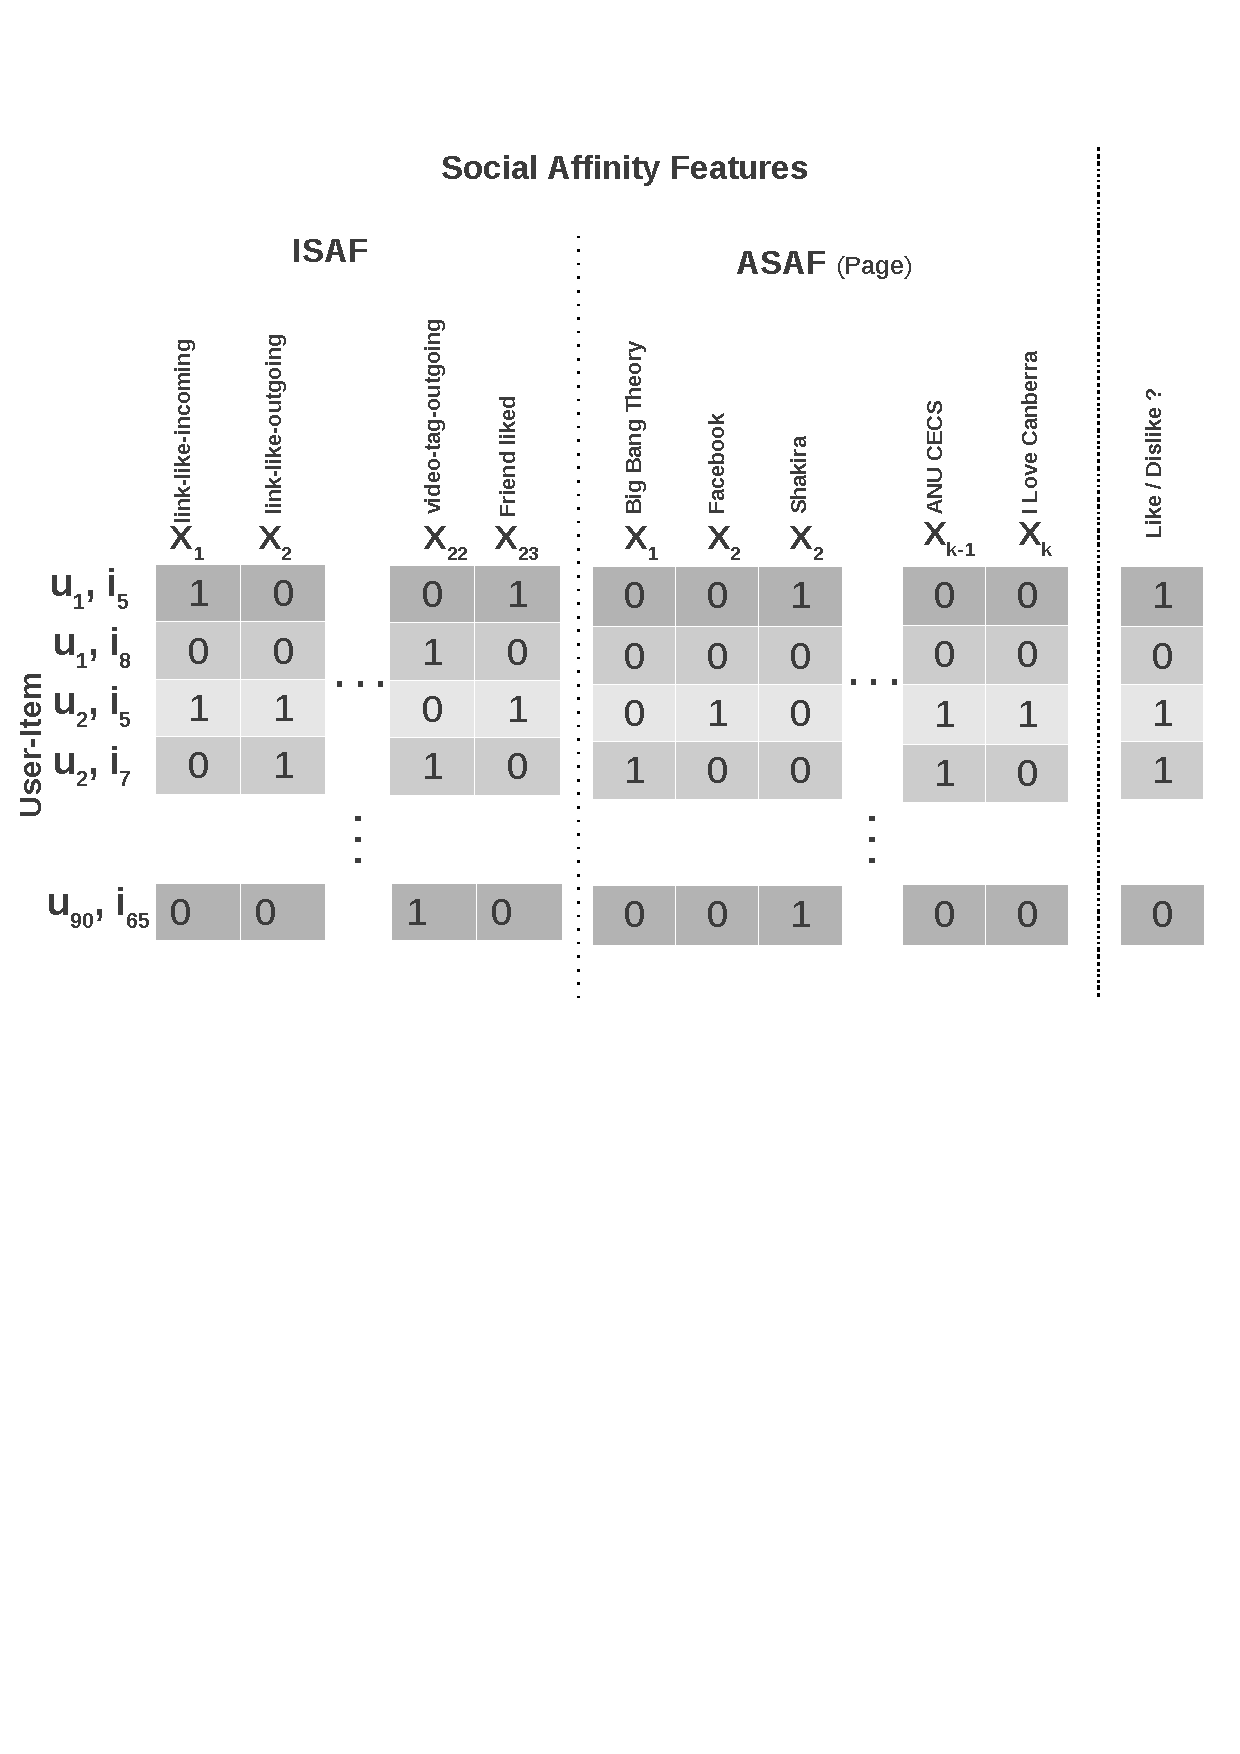
\includegraphics[width=1\linewidth]{data/plots/features/saf_features}
\caption{For each user-item, social affinity features\textit{(ASAF/ISAF)} are binary valued features which indicates
whether anyone from user's social affinity group\textit{(ISAG/ASAG)} liked the given item or not.}
\label{fig:features_overview}
\end{figure}
%#suvash#
%%%%%%%%%%%%%%%%%%%%%%%%%%%%%%%%%%%%%%%%%%%%%%%%%%%%%%%%%%%%%%%%%%%%%%

\emph{Social affinity filtering (SAF)} is a novel social
recommendation method that \emph{learns} which sets of social network
users --- defined via their fine-grained interactions and shared
activities with user $u$ --- are good proxies for $u$'s preference
over item $i$.  With the social affinity features as defined in
Sec~\ref{ssec:SAfeature} relying on SAGs as defined in
Sec~\ref{ssec:sag}, the task of SAF reduces to one of binary
classification.

Formally, given a user $u$ and item $i$, a SAF classifier is simply a
function 
\begin{equation*}
f: \x(u,i) \to \likes(u,i)
\end{equation*}
where we restrict $\likes(u,i) \in \{ \true, \false \}$\footnote{For
  training purposes, we omit any unobserved cases for which the class
  label $\likes(u,i)=\unknown$.  At prediction time, the binary
  classifier must always select a class label of $\true$ or $\false$.}
and specify a feature vector $\x(u,i) = \langle
\cdots,X^{u,i}_{k},\cdots \rangle$ over social affinity features
$k$.  To train $f$, one simply provides a dataset of historical
observations $D = \{ \x(u,i) \to \likes(u,i) \}$ where $f$ could be a
linear classifier trained by an SVM, logistic regression, or na\"{i}ve
Bayes.  For future predictions, we are simply given a new user $u$ and
item $i$ to predict for and build the feature vector $\x(u,i)$ from
which we can predict $\likes(u,i) = f(\x(u,i))$ using the trained
classifier $f$.

While a classification approach to recommendation might evoke
comparisons to \emph{content-based filtering} (CBF)~\cite{newsweeder},
we remark that CBF is not a \emph{social} recommendation approach and
unlike CBF, SAF does not require explicit user features (e.g., age,
gender, location, etc.) or item descriptors (link text, link genre,
etc.); in contrast, SAF uses interaction and/or activity data for
social network users to define SAGs and learns the affinities between
a user (ego) and the different set of alters as defined by these SAGs.
Additionally, unlike state-of-the-art \emph{social collaborative filtering} 
approaches~\cite{socinf,rrmf,ste,sorec,sr,Noel2012NOF,lla}, SAF does
not aggregate user-user interaction and shared activity data into a
single aggregate statistic, instead it uses fine-grained distinctions
in this social data to define a large number of SAGs and learns which
of these SAGs are informative for recommendation.


